\documentclass{standalone}

\usepackage{tikz}

\begin{document}
  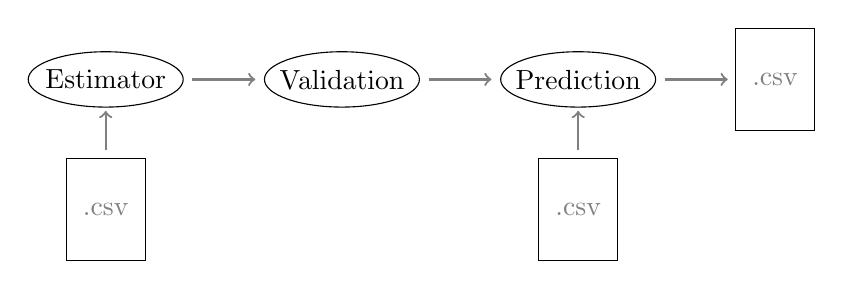
\begin{tikzpicture}
    \draw (-0.5, -2.3) rectangle (0.5, -1) node[midway, gray] {.csv};
    \draw [->, gray, thick] (0, -0.9) -- (0, -0.4);
    \draw (0, 0) ellipse (28pt and 10pt) node {Estimator};
    \draw [->, gray, thick] (1.1, 0) -- (1.9, 0);
    \draw (3, 0) ellipse (28pt and 10pt) node {Validation};
    \draw [->, gray, thick] (4.1, 0) -- (4.9, 0);
    \draw (6, 0) ellipse (28pt and 10pt) node {Prediction};
    \draw [->, gray, thick] (6, -0.9) -- (6, -0.4);
    \draw (5.5, -2.3) rectangle (6.5, -1) node[midway, gray] {.csv};
    \draw [->, gray, thick] (7.1, 0) --(7.9, 0);
    \draw (8, -0.65) rectangle (9, 0.65) node[midway, gray] {.csv};
  \end{tikzpicture}
\end{document}

